O aprendizado supervisionado é o campo dentro de aprendizado de máquina que visa a gerar modelos preditivos a partir de
um conjunto de dados de treinamento cujos resultados são previamente conhecidos.
Este capítulo apresentará as técnicas de aprendizado de máquina que serão utilizadas neste trabalho, ressaltando suas
aplicações no processamento de linguagem natural.

\section{Naïve Bayes} \label{sec:bayes}

Naïve Bayes é uma das técnicas mais simples disponíveis nesse contexto.
Ela se baseia no teorema de Bayes enquanto assume independência entre as características escolhidas para descrever o
dado.
Será demostrada sua formulação matemática, como descrita por Schütze~\cite{schutze08}.

Tendo $\mathbf{x}$ tal que $\mathbf{x} \in \mathbf{X}$ em que $\mathbf{X}$ é o conjunto de dados de treinamento, a sua
probabilidade de pertencer a classe $c_k \in \mathbf{c}$, sendo $\mathbf{c}$ o conjunto de classes, é dada pelo teorema de Bayes:
\begin{equation} \label{eq:bayes}
    p(c_k \mid \mathbf{x}) = \frac{p(c_k) \ p(\mathbf{x} \mid c_k)}{p(\mathbf{x})}
\end{equation}

Cada observação $\mathbf{x}$ é um vetor de $n$ características, e ao se assumir independência entre elas, obtém-se:
\begin{equation}
    p(x_i \mid x_{i+1}, \dots ,x_{n}, c_k ) = p(x_i \mid c_k)
\end{equation}

Logo, pode-se reescrever a Equação~\ref{eq:bayes} substituindo $p(\mathbf{x} \mid c_k)$ pelo produtório de suas
características:
\begin{equation}
    p(c_k \mid \mathbf{x}) = \frac{p(c_k) \prod_{i=1}^n p(x_i \mid c_k)}{p(\mathbf{x})}
\end{equation}

Como $p(\mathbf{x})$ será uma constante, dado cada exemplo $\mathbf{x}$ esta pode ser desprezada:
\begin{equation}
    p(c_k \mid \mathbf{x}) \propto p(c_k) \prod_{i=1}^n p(x_i \mid c_k)
\end{equation}

Portanto, tem-se que o estimador ótimo $\hat{y}$ escolherá pela classe que atinja maior probabilidade:
\begin{equation}
    \hat{y} = \underset{k \in \{1, \dots, K\}}{\operatorname{max}} \ p(c_k) \displaystyle\prod_{i=1}^n p(x_i \mid c_k)
\end{equation}

Vê-se então que o modelo de Naïve Bayes depende apenas de $p(c_k)$ e $p(\mathbf{x} \mid c_k)$.
Estes parâmetros serão extraídos do conjunto de treino por máxima verossimilhança.

Dado um vetor $\mathbf{y}$ de tamanho $m$ que represente as classificações referentes a $\mathbf{X}$, pode-se estimar
$p(c_k)$ pela contagem de vezes que a classe $c_k$ aparece no conjunto de treinamento:
\begin{equation}
    \hat{p}(c_k) = \frac{\sum_{i=1}^m [y_i = c_k]}{m}
\end{equation}

Por sua vez, $p(x_r \mid c_k)$ é estimado utilizando a contagem de vezes que uma característica aparece dividida pelo
total de características presentes no subconjunto $\mathbf{X'}$, subconjunto de dados de treinamento pertencentes a
classe $c_k$:
\begin{equation}
    \hat{p}(x_r \mid c_k) = \frac{\sum_{j=i}^{m'} \sum_{i=1}^n [x_{ji} = x_r]}{|\mathbf{X'}|}
\end{equation}

Vê-se que modelos montados a partir de Naïve Bayes são computacionalmente baratos, dado que seus parâmetros são
obtidos através de contagens sobre os dados de treinamento e que sua predição utiliza apenas multiplicações.
Embora se baseie na independência entre características, seu baixo custo operacional leva esta técnica a ser utilizada
mesmo em problemas com notória dependência entre características, como a classificação de texto~\cite{mccallum98}.

\section{Support Vector Machine}

O conceito fundamental do \textit{Support Vector Machine} (SVM) se dá pela obtenção de vetores de suporte que melhor
separe as classes.
Esta separação é feita de maneira que se maximize a margem entre as classes.
A Figura~\ref{fig:svm} demostra dados de duas classes distintas, representadas pelas cores rosa e amarelo, pertencentes
a um espaço de características de duas dimensões; vê-se na figura que a reta que define a maior separação é suportada
pelos dados de cada classe mais próximos a ela.

\begin{figure}
\begin{center} {
    \begin{center}
    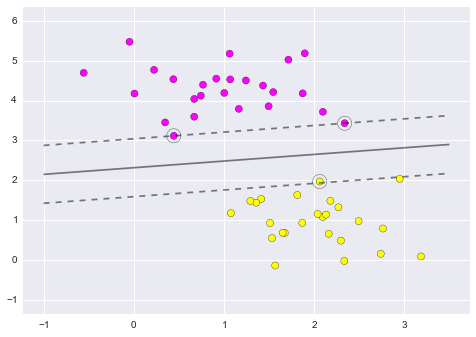
\includegraphics[scale=0.7]{svm.png}
    \caption{Reta de maior margem entre classes.}
    \small Imagem com direitos cedidos para uso não comercial, retirada de~\cite{vanderplas15}
    \label{fig:svm}
    \end{center}
}
\end{center}
\end{figure}

Como utilizam vetores de suporte para definir hiperplanos de separação, SVM não são capazes de segregar classes não
linearmente distinguíveis.
Podemos observar um exemplo deste caso na Figura~\ref{fig:svm-lin}, na qual uma SVM treinado tenta separar classes
concêntricas.
Para contornar esse impedimento, foi elaborado o que se chamou de \textit{kernel trick}.
Este se baseia em um mapeamento não linear dos dados para um espaço onde possam ser linearmente
separáveis~\cite{scholkopf02}.
A Figura~\ref{fig:svm-rbf} mostra a representação dos dados apresentados na Figura~\ref{fig:svm-lin} após seu mapeamento
por uma função de base radial.

\begin{figure}
\begin{center} {
    \begin{center}
    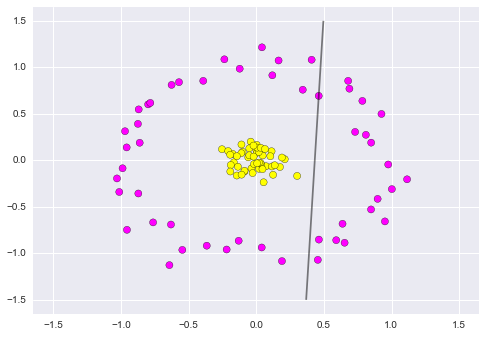
\includegraphics[scale=0.7]{svm-lin.png}
    \caption{SVM em dados não linearmente separáveis.}
    \small Imagem com direitos cedidos para uso não comercial, retirada de~\cite{vanderplas15}
    \label{fig:svm-lin}
    \end{center}
}
\end{center}
\end{figure}

\begin{figure}
\begin{center} {
    \begin{center}
    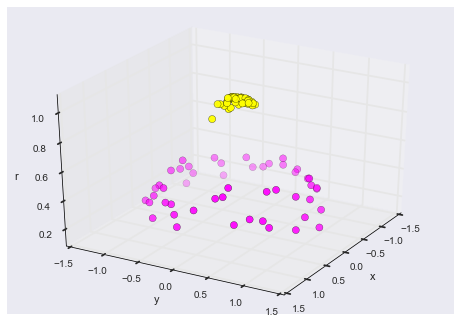
\includegraphics[scale=0.7]{svm-rbf.png}
    \caption{Transformação de dados por função de base radial.}
    \small Imagem com direitos cedidos para uso não comercial, retirada de~\cite{vanderplas15}
    \label{fig:svm-rbf}
    \end{center}
}
\end{center}
\end{figure}

Neste novo espaço definido pela transformação, os dados são linearmente separáveis.
Portanto, é possível achar um vetor de suporte que defina um hiperplano de separação das classes.
Vemos na Figura~\ref{fig:svm-rbf-clas} as margens encontradas.

\begin{figure}
\begin{center} {
    \begin{center}
    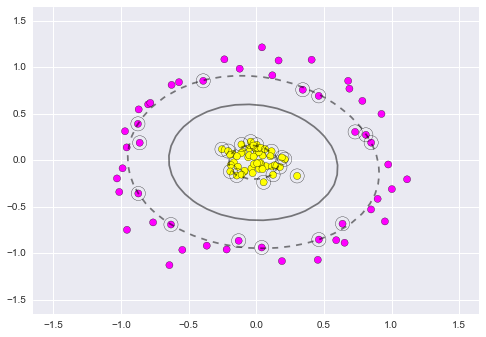
\includegraphics[scale=0.7]{svm-rbf-clas.png}
    \caption{SVM com \textit{kernel} de base radial.}
    \small Imagem com direitos cedidos para uso não comercial, retirada de~\cite{vanderplas15}
    \label{fig:svm-rbf-clas}
    \end{center}
}
\end{center}
\end{figure}

Porém, por se basear nos dados próximos ao limiar de separação das classes, o algoritmo é incapaz de distinguir os casos
de classes que não são separáveis sem erros.
A solução desse problema foi a criação de uma variável de relaxamento que define um número máximo de erros de
classificação permitido.
Esta propriedade é descrita com mais detalhes por Cortes e Vapnik em~\cite{cortes95}.
Sua utilização permite o desenvolvimento de modelos mais robustos a \textit{outliers} e melhora a generalização.
Outros exemplos de regularizadores, como este, serão apresentados na Subseção~\ref{sec:generalizacao}.

Uma limitação na utilização deste algoritmo é seu tempo de treinamento.
Sua complexidade computacional fica entre $O(n_{caracteristicas} \times n_{dados}^2)$ e
$O(n_{caracteristicas} \times n_{dados}^3)$~\cite{list09}.
Entretanto, Suykens e Vandewalle desenvolveram uma função custo através da qual tornou-se possível realizar o treinamento
de SVM a partir da otimização pelo método do gradiente~\cite{suykens99}, viabilizando sua utilização em ambientes com
limitações computacionais.

% falar de SVM aplicado a texto, kernel linear

\section{Redes Neurais} \label{sec:nn}

Redes neurais são sistemas computacionais que pretendem replicar o modelo de processamento do cérebro~\cite{wiener61}.
Inspirado pelo campo do conexionismo, em 1958 Rosenblatt~\cite{rosenblatt58} desenvolveu o algoritmo do perceptron.
O perceptron foi uma das primeiras formas de redes neurais desenvolvidas.
Eles são classificadores binários compostos por duas camadas de neurônios artificiais, uma de entrada e uma de saída,
interligados por sinapses.
As sinapses funcionam como um ponderador linear dos neurônios da camada anterior.
Os neurônios, por sua vez, representam uma função de ativação, no caso do perceptron a função degrau.
Porém, de maneira mais geral, dispõem de funções como: tangente hiperbólica, logística etc.

A utilização de perceptrons com múltiplas camadas sucessivas de neurônios formam as redes neurais
\textit{multilayer perceptron} (MLP), como exemplificado na Figura~\ref{fig:ff-neural-net}.
Nela, apresenta-se o diagrama de uma rede que conta com uma camada de entrada, a qual representa os dados do problema,
seguida de duas camadas intermediarias, comumente chamadas de escondidas, as quais são seguidas pela camada de saída,
que apontará o resultado final de todo processamento da rede.

\begin{figure}
\begin{center} {
    \begin{center}
    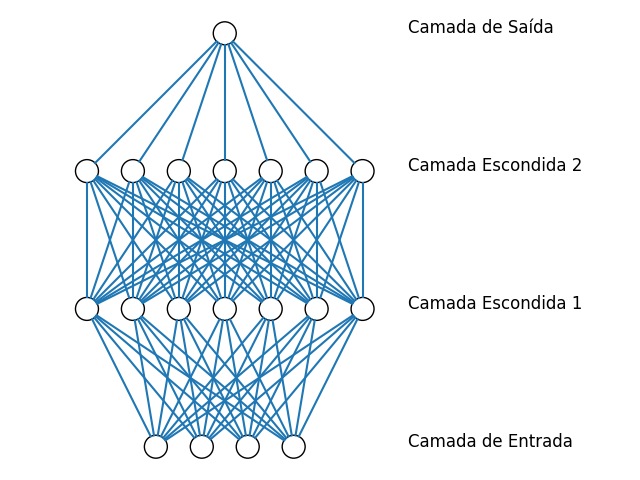
\includegraphics[scale=0.75]{ffnn.png}
    \caption{Rede neural \textit{multilayer perceptron}}
    \label{fig:ff-neural-net}
    \end{center}
}
\end{center}
\end{figure}

Uma de suas principais características de redes neurais é a capacidade de aproximar qualquer função, dado que a rede
contenha pelo menos uma camada escondida com número suficientemente grande de neurônios com ativação não
linear~\cite{hornik89}.

Porém, no final dos anos 60, Misky e Papert~\cite{minsky72} publicaram um estudo que prova que redes neurais com
apenas duas camadas, como o perceptron, são incapazes de realizar classificações não lineares.
Esta descoberta, junto com a inviabilidade computacional de se trabalhar com redes maiores na época, resultou em uma
estagnação dos estudos de redes neurais artificias.

Foi apenas em 1982, quando Werbos~\cite{werbos82} aplicou o método de otimização por auto diferenciação em redes neurais,
facilitando o aprendizado de redes de múltiplas camadas, que o estudo de redes neurais voltou a receber atenção.
Este método foi chamado de backpropagation.
Hinton \textit{et al.}~\cite{williams86} afirmam que este método é capaz de obter representações nas camadas
intermediárias que são apropriadas para resolução do problema em questão.

Será descrito a seguir um exemplo de treinamento por backpropagation aplicado a uma rede de uma camadas escondida e uma
saída.

A primeira etapa para utilização do backpropagation é computar o valor previsto ${\hat{y}_i}$ pela rede neural, para
uma dada observação de índice $i$ do conjunto de treinamento, como descrito nas
equações~\crefrange{eq:nn-forward-a1}{eq:nn-forward-y}.
Nelas, $f$ representa a função de ativação; $\mathbf{x}_i$ o conjunto de características que descreve esse exemplo;
$\mathbf{W}$ e $\mathbf{b}$ os pesos e o \textit{bias} respectivamente; e $\mathbf{h}_i$ indica a camada escondida.

\begin{subequations} \label{eq:nn-forward}
\begin{align}
    &\mathbf{a}_i^{(1)} = \mathbf{W}^{(1)} \mathbf{x}_i + \mathbf{b}^{(1)} \label{eq:nn-forward-a1}\\
    &\mathbf{h}_i = f(\mathbf{a}_i^{(1)}) \label{eq:nn-forward-hidden}\\
    &a_i^{(2)} = \mathbf{W}^{(2)} \mathbf{h}_i + b^{(2)} \label{eq:nn-forward-a2}\\
    &\hat{y}_i = f(a_i^{(2)}) \label{eq:nn-forward-y}
\end{align}
\end{subequations}

Em seguida, utiliza-se uma função custo $L$ para calcular o erro $J$ de representação obtido pela rede neural a partir
das previsões $\mathbf{\hat{y}}$ e das anotações $\mathbf{y}$, como exposto na Equação~\ref{eq:nn-cost}.
A Seção~\ref{sec:custo} apresenta exemplos de funções custo.

\begin{equation} \label{eq:nn-cost}
    J_i = L(\hat{y}_i, y_i)
\end{equation}

A computação do custo $J$ conclui a parte \textit{forward} do algoritmo, no qual os valores das saídas de cada camada da
rede são armazenados para execução da etapa seguinte, a \textit{backward}.
Na fase \textit{backward}, utiliza-se o gradiente do erro da rede neural em relação a cada camada para ponderar quanto
cada peso influi no erro de representação.
Desta maneira, parâmetros que estejam menos adaptados ao problema receberão os maiores gradientes, e consequentemente os
maiores ajustes, visto que são os mais responsáveis pelo erro.

As equações~\crefrange{eq:nn-backprop-a2}{eq:nn-backprop-b1} mostram a propagação do gradiente a partir da camada de
saída até a camada de entrada, utilizando-se os valores de $\mathbf{a}_i$ previamente obtidos.
Dispondo do gradiente da função custo em relação a saída, $\frac{\partial{J_i}}{\partial{y_i}}$, que é dependente da
função escolhida, calcula-se por regra da cadeia o gradiente do erro em relação aos pesos e \textit{bias} da camada de
saída, como observa-se nas equações~\cref{eq:nn-backprop-w2,eq:nn-backprop-b2}.
Computa-se também o gradiente da camada escondida, como apresentado na Equação~\ref{eq:nn-backprop-h}.
Uma vez apurado o gradiente da camada escondida, pode-se calcular os gradientes dos pesos e \textit{bias} desta camada
como presentes nas equações~\cref{eq:nn-backprop-w1,eq:nn-backprop-b1}.

\begin{subequations} \label{eq:nn-backprop}
\begin{align}
    &\frac{\partial{J_i}}{\partial{a_i^{(2)}}}
        = \frac{\partial{J_i}}{\partial{y_i}} \frac{\partial{y_i}}{\partial{a_i^{(2)}}}
        = \frac{\partial{J_i}}{\partial{y_i}} f^{\prime}(a_i^{(2)}) \label{eq:nn-backprop-a2}\\
    &\frac{\partial{J_i}}{\partial{\mathbf{W}^{(2)}}}
        = \frac{\partial{J_i}}{\partial{a_i^{(2)}}} \frac{\partial{a_i^{(2)}}}{\mathbf{W}^{(2)}}
        = \frac{\partial{J_i}}{\partial{a_i^{(2)}}} \mathbf{h}_i \label{eq:nn-backprop-w2}\\
    &\frac{\partial{J_i}}{\partial{b^{(2)}}}
        = \frac{\partial{J_i}}{\partial{a_i^{(2)}}} \frac{\partial{a_i^{(2)}}}{\partial{b^{(2)}}}
        = \frac{\partial{J_i}}{\partial{a_i^{(2)}}} \label{eq:nn-backprop-b2}\\
    &\frac{\partial{J_i}}{\partial{\mathbf{h}_i}}
        = \frac{\partial{J_i}}{\partial{a_i^{(2)}}} \frac{\partial{a_i^{(2)}}}{\partial{\mathbf{h}_i}}
        = \frac{\partial{J_i}}{\partial{a_i^{(2)}}} \mathbf{W}^{(2)} \label{eq:nn-backprop-h}
\end{align}

\begin{align}
    &\frac{\partial{J_i}}{\partial{\mathbf{a}_i^{(1)}}}
        = \frac{\partial{J_i}}{\partial{\mathbf{h}_i}} \frac{\partial{\mathbf{h}_i}}{\partial{\mathbf{a}_i^{(1)}}}
        = \frac{\partial{J_i}}{\partial{\mathbf{h}_i}} f^{\prime}(\mathbf{a}_i^{(1)})\\
    &\frac{\partial{J_i}}{\partial{\mathbf{W}^{(1)}}}
        = \frac{\partial{J_i}}{\partial{\mathbf{a}_i^{(1)}}} \frac{\partial{\mathbf{a}_i^{(1)}}}{\mathbf{W}^{(1)}}
        = \frac{\partial{J_i}}{\partial{\mathbf{a}_i^{(1)}}} \mathbf{x}_i \label{eq:nn-backprop-w1}\\
    &\frac{\partial{J_i}}{\partial{\mathbf{b}^{(1)}}}
        = \frac{\partial{J_i}}{\partial{\mathbf{a}_i^{(1)}}} \frac{\partial{\mathbf{a}_i^{(1)}}}{\mathbf{b}^{(1)}}
        = \frac{\partial{J_i}}{\partial{\mathbf{a}_i^{(1)}}} \label{eq:nn-backprop-b1}
\end{align}
\end{subequations}

Os gradientes dos pesos e \textit{bias} serão utilizados para sua otimização pelo método do gradiente objetivando a
minimizar a função custo.
A Seção~\ref{sec:optimizers} aborda o tema de otimizadores, focando em rede neurais.

\subsection{Deep Learning}

O aumento do poder computacional ao longo dos anos levou à utilização de redes neurais mais robustas.
Todavia, a adição de múltiplas camadas a redes neurais feedforward apresenta dificuldades no treinamento por
\textit{backpropagation} pelo efeito do \textit{vanishing gradient}~\cite{hochreiter98}.
O \textit{vanishing gradient} acontece quando os pesos das camadas mais externas da rede são treinados até o ponto em
que o gradiente dos seus erros sejam pequenos.
A partir desse momento, as camadas mais próximas da entrada recebem atualizações menores em seus pesos, visto que o fator
de atualização depende da multiplicação dos gradientes das camadas mais externas.
Este processo resulta no treinamento efetivo apenas das camadas próximas à saída, estabelecendo uma dificuldade
exponencial no treinamento com relação ao número de camadas.

Foi somente quando Hinton \textit{et al.} desenvolveram o pré-treinamento camada a camada~\cite{hinton06} que o problema
do \textit{vanishing gradiente} começou a ser contornado, viabilizando a aplicação de redes neurais feedforward com muitas
camadas.
Essa técnica consiste em se obter um conjunto de pesos de cada camada de neurônios individualmente de maneira a melhor
representar a sua entrada, de forma que posteriormente esse conjunto de pesos sirva como inicialização para o
treinamento da rede.
Outros métodos de redução do \textit{vanishing gradiente} são utilizados, como a função de ativação ReLU
(\textit{rectified linear unit})~\cite{nair10} e, mais recentemente, as arquiteturas de redes neurais
residuais~\cite{he16}.

Chamou-se de \textit{Deep Learning} o campo de estudo de redes neurais com muitas camadas.
Redes neurais profundas romperam barreiras de performance em problemas como reconhecimento de fala, detecção de
objetos, tradução etc~\cite{lecun15}.

Cada camada de uma rede neural gera uma abstração que representa a sua entrada de modo a facilitar a tarefa a ser
realizada.
O encadeamento de camadas resulta em representações mais complexas dos dados, revelando relações previamente não
observáveis.
O aprofundamento das redes tem como consequência a redução ou eliminação da chamada \textit{feature engineering},
processo de seleção de características que usualmente requer expertise no domínio do problema.
Considerando por exemplo o caso do diagnóstico de câncer de pele, técnicas tradicionais de classificação dependiam de
extração de informações de imagens de lesões, tais como: formato, tamanho, cor etc.
Modelos baseados em redes neurais profundas são capazes de obter resultados superiores, eliminando completamente esta
etapa~\cite{esteva17}.

Contudo, as técnicas de \textit{Deep Learning} não se limitam apenas à arquitetura \textit{multilayer perceptron}.
Dentre as arquiteturas frequentemente utilizadas, tem-se: redes neurais recursivas (RNN)~\cite{hopfield87}, redes neurais
convolucionais, \textit{autoencoders}~\cite{hinton06_2} e redes neurais geradoras adversárias
(GAN)~\cite{goodfellow14_2}.
A Seção~\ref{sec:convolucionais} apresenta detalhes das redes neurais convolucionais, técnica aplicada neste trabalho.

\subsection{Redes Neurais Convolucionais} \label{sec:convolucionais}

A utilização de redes neurais \textit{multilayer perceptron} em imagens sofre limitações.
Por cada pixel estar diretamente ligado aos neurônios, rotações ou translações na imagem afetam fortemente a capacidade
da rede.
Pretendendo solucionar estes problemas, foram desenvolvidas redes neurais convolucionais, cujas conexões são baseadas
no funcionamento do córtex visual.

Elas são compostas primariamente de dois tipos de camadas: convolucionais e \textit{pooling}.
Camadas convolucionais são formadas por um conjunto de filtros espaciais compostos das mesmas funções não-lineares
utilizadas em redes MLP~\cite{goodfellow16}.
Para cada exemplo do conjunto de dados, o filtro, cujo tamanho é menor que a entrada, é aplicado no inicio do dado e
deslocado até o final.
Desta forma, os filtros dividem os pesos entre todo espaço do dado, permitindo uma insensibilidade a deslocamentos e
rotações.
Por sua vez, as camadas de \textit{pooling} tem como objetivo reduzir o número total de sinapses da rede.
Para tal, reduz-se o tamanho dos filtros, obtendo-se valores máximos ou médios de dimensões desses filtros.
\textit{Pooling} é fundamental quando o objetivo a ser atingido depende mais da presença de uma característica do que
sua posição no dado~\cite{goodfellow16}.

Apesar de Redes Convolucionais terem sido desenvolvidas com intuito de solucionar problemas de visão computacional, elas
também obtiveram êxito nas mais diversas áreas, como no reconhecimento de voz e em séries temporais~\cite{lecun95}.
Tal sucesso pode ser atribuído à insensibilidade da rede a deslocamentos.

Kim~\cite{kim14}, por sua vez, propôs o uso de redes convolucionais aplicadas a texto.
Para tal, os documentos são representados em uma matriz na qual cada coluna é composta pelos pesos de um
\textit{embedding}, como o Word2Vec, correspondente a cada palavra.
Por cada mensagem poder ter tamanho variado, escolhe-se um número de tokens $n$, para representar cada mensagem.
Dos documentos que contêm número de palavras maior do que o escolhido, selecionam-se os $n$ primeiros tokens.
Nos casos em que a mensagem é menor, ela é completada com tokens de preenchimento, os quais são alocados na origem do
espaço do \textit{embedding}.
O número $n$ é escolhido com base nos dados disponíveis de treinamento, de maneira a não se desperdiçar grande
quantidade de informação, nem se fazer uso excessivo dos tokens.

A principal diferença na utilização de redes convolucionais em texto é que nesse caso as convoluções e \textit{poolings}
são operadas em apenas uma dimensão, a dimensão que representa a posição de cada palavra na mensagem.
Desta maneira, cada filtro se desloca apenas entre as janelas de tokens, englobando toda a representação do
\textit{embedding} de cada token.

\section{Funções Custo} \label{sec:custo}

Dá-se o nome de função custo às funções que caracterizam a distância entre o resultado obtido pela rede e seu objetivo.
Assim, as sinapses de redes neurais são otimizadas a partir da minimização de tais funções.
Nesta seção, serão apresentadas as funções custo mais relevantes no contexto de redes neurais.

\subsection{Erro Médio Quadrático}

A função custo mais utilizada é o erro médio quadrático (EMQ).
Seu fator quadrático pune mais severamente grandes erros, acelerando o processo de otimização.

A fórmula~\ref{eq:mse} mostra a composição do EMQ, sendo $n$ o número de pares de exemplos e $\hat{y}$ a predição da
rede neural.

\begin{equation} \label{eq:mse}
    \frac{\displaystyle\sum^n |\hat{\mathbf{y}}_i - \mathbf{y}_i|^2}{n}
\end{equation}

\subsection{Erro Médio Absoluto}

O erro médio absoluto se assemelha ao EMQ, tendo como diferença a falta do fator quadrático, conforme observa-se na fórmula~\ref{eq:mae}.

\begin{equation} \label{eq:mae}
    \frac{\displaystyle\sum^n |\hat{\mathbf{y}}_i - \mathbf{y}_i|}{n}
\end{equation}

\subsection{Erro Médio Absoluto Percentual}

Há situações em que se pretende mapear um objetivo com extensão de diferentes ordens de grandeza. O uso de erro médio quadrático ou absoluto nestes casos irá dar menos relevância a entradas pequenas. Para solucionar este problema, o erro médio absoluto percentual é composto conforme apresentado na fórmula~\ref{eq:mape}

\begin{equation} \label{eq:mape}
    \frac{100}{n}\sum^n \left|\frac{\hat{\mathbf{y}}_i - \mathbf{y}_i}{\mathbf{y}_i}\right|
\end{equation}

\subsection{Entropia Cruzada}

A entropia cruzada é uma medida que contém a distância entre duas distribuições de probabilidades. Sua formula é disposta de maneira que sua otimização encontre os parâmetros de máxima verossimilhança. As equações~\ref{eq:likelihood-label} e~\ref{eq:likelihood-map} mostram a dedução da função de verossimilhança $\mathcal{L}$ a partir da probabilidade a posteriori, na qual $k$ representa cada classe presente no conjunto de dados.

\begin{equation} \label{eq:likelihood-label}
    \mathcal{L}(\theta) = \prod_k P(\mathbf{y}_k \mid \mathbf{x})
\end{equation}

\begin{equation} \label{eq:likelihood-map}
    \mathcal{L}(\theta) = \prod_k \mathbf{\hat{y}}_k^{\mathbf{y}_k} (1 - \mathbf{\hat{y}}_k)^{(1 - \mathbf{y}_k)}
\end{equation}

Para simplificar o custo computacional, o valor máximo da função verossimilhança é obtido minimizando-se o negativo de seu logaritmo, como presente na fórmula~\ref{eq:loglikelihood}.

\begin{equation} \label{eq:loglikelihood}
        -\ln(\mathcal{L}(\theta)) = -\sum_k \mathbf{y}_k \ln(\mathbf{\hat{y}}_k) + (1 - \mathbf{y}_k) \ln(1 - \mathbf{\hat{y}}_k)
\end{equation}

A expressão~\ref{eq:cec} mostra o uso da entropia cruzada como função custo. A segunda parte do somatório determina que a acurácia de não classe pode ser ignorada para determinada classe $k$, visto que esta já será considerada na sua classe correta. É necessário notar que a sua utilização depende de $\mathbf{y}_i$ e $\hat{\mathbf{y}_i}$ serem limitados entre 0 e 1. Para adequar-se a esta limitação, caso a rede neural possua apenas uma saída, utiliza-se ativação Sigmoid na última camada. Em caso de múltiplas saídas, utiliza-se ativação Softmax.

\begin{equation} \label{eq:cec}
    \frac{-\displaystyle\sum^n \sum_k \mathbf{y}_k \ln(\mathbf{\hat{y}}_k)}{n}
\end{equation}

\section{Otimizadores} \label{sec:optimizers}

Definidas as funções custo, nesta seção serão abordados os algoritmos responsáveis por sua minimização.
Embora a área de otimização apresente uma vasta gama de opções, sua utilização em aprendizado de máquina costuma se
restringir a algoritmos de primeira ordem, como o gradiente descendente, principalmente por seu menor custo
computacional.
O método do gradiente, primeiramente apresentado por Cauchy em 1847~\cite{cauchy1847}, consiste em minimizar a função
custo por meio de atualizações iterativas de parâmetros do modelo, a partir da derivada da própria função custo em
relação aos parâmetros.

Redes neurais, em geral, possuem funções custo não convexas.
Assim sendo, o algoritmo de gradiente descendente não garante convergência ao mínimo global.
A convergência a mínimos locais torna o modelo sensível a parâmetros, como funções de ativação, número de neurônios,
etc., e o torna sensível também à inicialização dos pesos, como mostra Glorot no artigo em que apresenta um método
homônimo de inicialização de pesos ~\cite{glorot10}.
Entretanto, o problema de convergência não se limita a mínimos locais.
Dauphin~\cite{dauphin14} mostra que quanto maior o número de variáveis latentes do modelo, maior a proporção de pontos
de sela em relação a mínimos locais.
Mostra também que os mínimos locais estão mais propensos a aparecer em pontos críticos com baixo custo, enquanto pontos
de sela costumam aparecer em pontos de alto custo.
Goodfellow~\cite{goodfellow14} apresenta resultados empíricos da efetividade do método do gradiente na fuga dos pontos
de sela.

O Algoritmo~\ref{al:gd} descreve a forma tradicional do gradiente descendente, dado que $L$ é a função custo adotada e
que $\mathbf{\hat{y}}$ é o mapeamento obtido pela rede neural a partir dos dados $\mathbf{x}$ e pesos
$\boldsymbol{\theta}$.
Observa-se que $\mathbf{\hat{g}}$ é a estimativa do gradiente dos pesos obtida a partir dos dados de treinamento.

\begin{algorithm}
    \caption{Gradiente Descendente}
    \label{al:gd}
    \begin{algorithmic}[1]
        \Require Taxa de treinamento $\epsilon$
        \Require Pesos iniciais $\boldsymbol{\theta}_{0}$
        \Require Número de iterações $T$

        \State $t \gets 0$
        \While {$t < T$}
            \State $t \gets t + 1$
            \State $\mathbf{\hat{y}} \gets f(\mathbf{x}, \boldsymbol{\theta}_{t-1})$
            \State $\mathbf{\hat{g}} \gets \frac{1}{n} \nabla_{\boldsymbol{\theta}} \sum_i^n L(\mathbf{\hat{y}}^{(i)}, \mathbf{y}^{(i)})$
            \State $\boldsymbol{\theta}_{t} \gets \boldsymbol{\theta}_{t-1} - \epsilon \mathbf{\hat{g}}$
        \EndWhile
    \end{algorithmic}
\end{algorithm}

Serão apresentadas nas próximas subseções as variações do método do gradiente mais notórias no treinamento de redes
neurais.

\subsection{Gradiente Descendente Estocástico}

A forma canônica do algoritmo do gradiente descendente começa a apresentar dificuldades de utilização em conjuntos de
dados de tamanho considerável.
Como observa-se no Algoritmo~\ref{al:gd}, para cada atualização dos pesos $\boldsymbol{\theta}$ é necessária a
estimação do gradiente $\mathbf{\hat{g}}$, a qual, por sua vez, depende da computação da função custo sobre todos os
dados.
Além do alto custo computacional, bases de dados grandes tendem a conter várias instâncias de dados muito próximos, não
adicionando significativamente informação à estimação do gradiente.

Uma das soluções deste problema, abordada pelo \textit{Gradiente Descendente Estocástico}, é a divisão do conjunto de
treinamento em lotes, nos quais serão estimados os gradientes.
Cada interação sobre o conjunto inteiro de dados é chamada de época e entre cada época costuma-se embaralhar os dados.
Já as outras partes do algoritmo permanecem iguais à implementação tradicional, como apresentado em~\ref{al:gd}.

\subsection{Gradiente Descendente com Momento}

A escolha da taxa de treinamento envolve uma troca entre tempo de treinamento e grau de convergência.
Altas taxas de treinamento podem apresentar dificuldades de convergência ou comportamentos oscilatórios em torno de um
ponto de custo mínimo, enquanto baixas taxas de treinamento consomem muito tempo de treinamento em regiões de alto
custo, diminuindo assim sua viabilidade.
Objetivando-se obter um melhor compromisso, foi acrescentado o momento ao método do gradiente, como formulado no
Algoritmo~\ref{al:gdm}.
O termo adicional $\mathbf{v}$ representa a "velocidade" do gradiente e a constante de momento $\alpha$ condiz com a
taxa de decaimento exponencial do termo $\mathbf{v}$.

\begin{algorithm}
    \caption{Gradiente Descendente com Momento}
    \label{al:gdm}
    \begin{algorithmic}[1]
        \Require Taxa de treinamento $\epsilon$
        \Require Constante de momento $\alpha$
        \Require Pesos iniciais $\boldsymbol{\theta}_{0}$
        \Require Número de iterações $T$

        \State $t \gets 0$
        \State $\mathbf{v}_{0} \gets \vec{0}$
        \While {$t < T$}
            \State $t \gets t + 1$
            \State $\mathbf{\hat{y}} \gets f(\mathbf{x}, \boldsymbol{\theta}_{t-1})$
            \State $\mathbf{\hat{g}} \gets \frac{1}{n} \nabla_{\boldsymbol{\theta}} \sum_i^n L(\mathbf{\hat{y}}^{(i)}, \mathbf{y}^{(i)})$
            \State $\mathbf{v}_{t} \gets \alpha \mathbf{v}_{t-1} - \epsilon \mathbf{\hat{g}}$
            \State $\boldsymbol{\theta}_{t} \gets \boldsymbol{\theta}_{t-1} + \mathbf{v}_t$
        \EndWhile
    \end{algorithmic}
\end{algorithm}

O momento permite que, enquanto o gradiente $\mathbf{\hat{g}}$ mantiver o mesmo sinal entre iterações, o módulo da
velocidade $\mathbf{v}$ cresça, acelerando o processo de aprendizado.
Quando o sinal do gradiente for invertido, ou seja, passar de um ponto de custo mínimo, o módulo da velocidade será
reduzido até seu sentido ser revertido, voltando ao mínimo.
Segundo Haykin~\cite{haykin09}, o uso do momento tem um efeito estabilizador no algoritmo de aprendizado.

\subsection{Adam}

Outra abordagem adotada nos algoritmos de otimização é o ajuste da taxa de aprendizado de maneira independente para
cada dimensão do espaço.
Duchi \textit{et al.}~\cite{duchi11} propuseram o algoritmo \textit{AdaGrad} (\textit{Adaptative Gradient}), no qual a
regra de atualização dos pesos é inversamente proporcional à soma do gradiente ao quadrado em todas as iterações
anteriores.
Dessa forma, direções que tenham grandes e frequentes atualizações serão amortecidas rapidamente, enquanto dimensões com
raras atualizações mantêm seu treinamento significativo por mais iterações.
Algoritmos com taxa de treinamento adaptativo, como o proposto por Duchi \textit{et al.}, atingem bons resultados em
problemas com dimensões esparsas, como o exemplo de Pennington \textit{et al.}~\cite{pennington14} no treinamento de
\textit{embeddings} de palavras, técnica que será apresentada na Seção~\ref{sec:w2v}.

Kingma e Ba~\cite{kingma14} projetaram o algoritmo \textit{Adam}, \textit{adaptative moment estimation}, baseado nos
princípios do \textit{AdaGrad}.
\textit{Adam} estima o primeiro e o segundo momentos do gradiente, média e variância não centralizada, a partir da média
móvel de ambos.
A regra de atualização de pesos é controlada pela taxa de treinamento $\epsilon$, e pelas estimativas de média e
variância, $\mathbf{\hat{m}}$ e $\mathbf{\hat{v}}$ respectivamente, dada a fórmula
$\boldsymbol{\theta}_{t} \gets \boldsymbol{\theta}_{t-1} - \epsilon \frac{\mathbf{\hat{m}}_{t}}{\sqrt{\mathbf{\hat{v}}_{t}}}$.
Portanto, gradientes grandes por seguidas iterações aumentam a média e, por consequência, o tamanho do passo.
Por sua vez, altas variâncias forçam a diminuição da taxa efetiva de aprendizado.

O Algoritmo~\ref{al:adam} possui a implementação de \textit{Adam} em pseudocódigo.
Os valores dos decaimentos betas costumam ser escolhidos em torno de 0,9 para $\beta_{1}$ e 0,999 para $\beta_{2}$.
Pelos momentos serem inicializados em zero, é necessário corrigir a tendência para se obter a verdadeira estimativa.

\begin{algorithm}
    \caption{Adam}
    \label{al:adam}
    \begin{algorithmic}[1]
        \Require Taxa de treinamento $\epsilon$
        \Require Constante de decaimento $\beta_{1}, \beta_{2}$
        \Require Pesos iniciais $\boldsymbol{\theta}_{0}$
        \Require Número de iterações $T$

        \State $t \gets 0$
        \State $\mathbf{m}_{0} \gets \vec{0}$
        \State $\mathbf{v}_{0} \gets \vec{0}$
        \While {$t < T$}
            \State $t \gets t + 1$
            \State $\mathbf{\hat{y}} \gets f(\mathbf{x}, \boldsymbol{\theta}_{t-1})$
            \State $\mathbf{\hat{g}} \gets \frac{1}{n} \nabla_{\boldsymbol{\theta}} \sum_i^n L(\mathbf{\hat{y}}^{(i)}, \mathbf{y}^{(i)})$
            \State $\mathbf{m}_{t} \gets \beta_{1} \mathbf{m}_{t-1} + (1 - \beta_{1}) \mathbf{\hat{g}}$
            \State $\mathbf{v}_{t} \gets \beta_{2} \mathbf{v}_{t-1} + (1 - \beta_{2}) \mathbf{\hat{g}}^{2}$
            \State $\mathbf{\hat{m}}_{t} \gets \frac{\mathbf{m}_{t}}{(1 - \beta_{1}^{t})}$
            \State $\mathbf{\hat{v}}_{t} \gets \frac{\mathbf{v}_{t}}{(1 - \beta_{2}^{t})}$
            \State $\boldsymbol{\theta}_{t} \gets \boldsymbol{\theta}_{t-1} - \epsilon \frac{\mathbf{\hat{m}}_{t}}{\sqrt{\mathbf{\hat{v}}_{t}}} $
        \EndWhile
    \end{algorithmic}
\end{algorithm}

\textit{Adam} apresenta robustez à escolha da taxa de treinamento $\epsilon$, visto que esta funciona como um limite
superior da taxa efetiva de atualização dos pesos, conforme provado em seu artigo~\cite{kingma14}, juntamente com sua
análise de convergência e com seus resultados experimentais.
Por se utilizar de médias móveis na estimação dos momentos, o algoritmo apresenta outra vantagem, sua capacidade de se
adaptar a funções objetivos não estacionárias.

Por sua robustez à escolha de hiperparâmetros e por sua aceleração do processo de aprendizado, \textit{Adam} se tornou
uma das principais técnicas de otimização de redes neurais profundas.

\section{Generalização} \label{sec:generalizacao}

Um dos principais fatores de um sistema de aprendizado de maquina é sua capacidade de generalizar.
isto acontece quando seu desempenho em dados de teste, ou seja, dados que não foram utilizados na fase de treinamento,
é equivalente ou suficientemente próximo ao obtido durante o aprendizado.

A fase de aprendizado do sistema pode ser vista como o processo de ajuste de parâmetros.
Desta forma, ao tentar representar a função, o modelo pode sofrer com sobreajuste, \textit{overfitting}, adequando-se
demais aos dados de treinamento.
O oposto também acontece quando o modelo é incapaz de mapear a complexidade entre as entradas e a saída.
A este evento dá-se o nome de subajuste, \textit{underfit}.
Tais eventos estão exemplificados na Figura~\ref{fig:fitting}.


\begin{figure}
\begin{center} {
    \begin{center}
    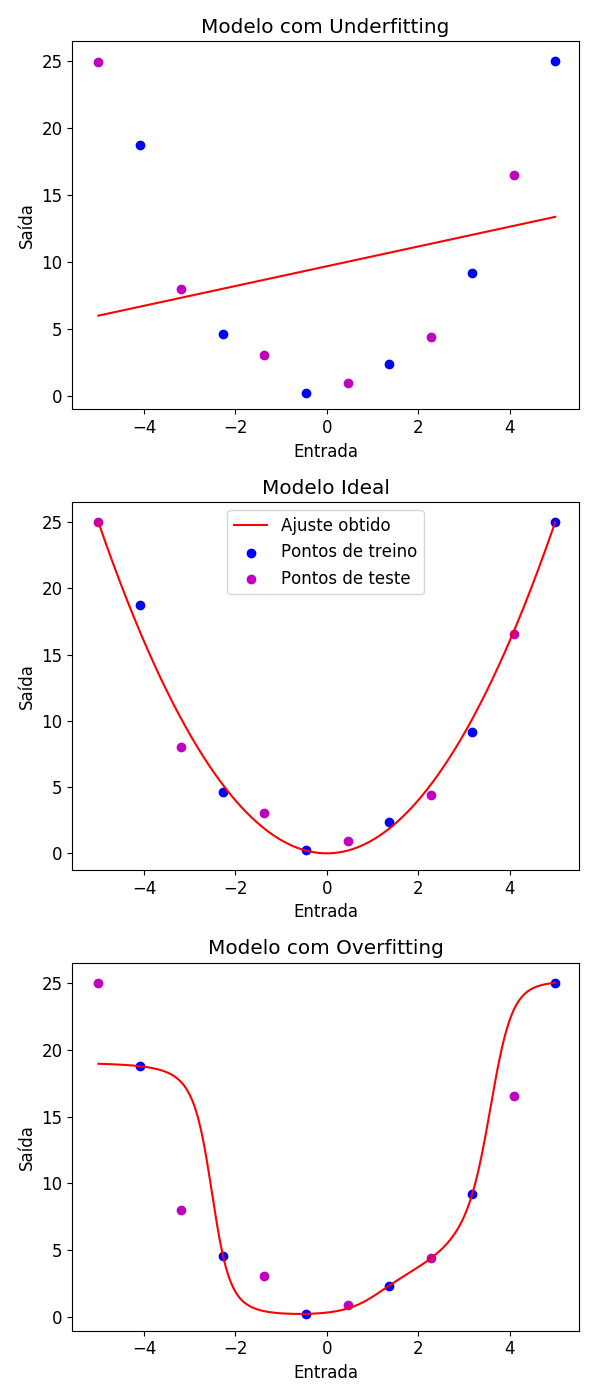
\includegraphics[scale=0.4]{fitting.png}
    \caption{Diferentes pontos de ajuste dos algoritmos de aprendizado de máquina.}
    \label{fig:fitting}
    \end{center}
}
\end{center}
\end{figure}

O uso de modelos robustos como os de \textit{Deep Learning} implica em uma maior propensão de se obter
\textit{overfitting} durante o treinamento, resultado de seu crescente número de parâmetros livres.
Abordando esse problema, foi desenvolvido um conjunto de técnicas que visam a reduzir o \textit{overfitting}, conjunto
esse que recebe o nome de regularização.
Nas subseções seguintes serão apresentadas as duas principais técnicas de regularização.

\subsection{Regularização de Tikhonov}

As regularizações de norma compõem um dos grupos mais simples de regularização.
Seu funcionamento é possível pois se adiciona à função custo um termo proporcional aos pesos, penalizando neurônios
com grandes normas.
Assim, limita-se a capacidade do modelo e, consequentemente, diminui-se o potencial de \textit{overfitting}.

Também conhecida como regularização $L_{2}$, a regularização de Tikhonov utiliza-se da norma quadrática dos pesos.
A formula~\ref{eq:custo-l2} exemplifica a função custo erro médio quadrático com o termo adicional de regularização
$L_{2}$, que por sua vez é controlado por uma constante $\lambda$.

\begin{equation} \label{eq:custo-l2}
    \frac{\displaystyle\sum^n |\hat{\mathbf{y}}_i - \mathbf{y}_i|^2}{n} + \frac{\lambda}{2} \lVert \boldsymbol{\theta} \rVert_{2}^{2}
\end{equation}

Krogh e Hertz~\cite{krogh92} provam que o uso de regularização $L_{2}$ é capaz de suprimir parâmetros irrelevantes,
diminuindo o número de parâmetros do modelo, e de reduzir o efeito de ruídos presentes na anotação dos dados.

\subsection{Dropout}
% substituir neuronio por outras palavras

Apresentado por Srivastava \textit{et al.}~\cite{srivastava14}, \textit{Dropout} é um método que propõe reduzir o
\textit{overfitting} por meio do desligamento temporário e aleatório de neurônios durante a etapa de treinamento.
Esse processo dá-se pela escolha de um parâmetro fixo $p$ que define a probabilidade de manutenção de cada neurônio.
A partir desse ponto, se desconectam os neurônios sorteados, efetivamente multiplicando seus pesos por 0 e resultando
em uma rede neural composta por um subconjunto de pesos da rede original, pesos esses que serão treinados com
\textit{Backpropagation}, como habitual.
Os sorteios ocorrem a cada seleção de lote do algoritmo do gradiente, levando a se treinar um número exponencial de
redes neurais durante a fase de aprendizado.
\textit{Dropout} pode ser aplicado tanto em neurônios de camadas escondidas, como em neurônios de entrada.
Os valores de $p$ são costumeiramente escolhidos por volta de $0,5$ para camadas escondidas e $0,8$ para camadas de
entrada.

\textit{Dropout} se deriva de um conjunto de técnicas de combinação de modelos, também conhecidas como
\textit{ensembling}.
Como mostra Dietterich \textit{et al.}~\cite{dietterich00}, modelos significativamente diferentes, quando combinados,
costumam resultar em melhoras na performance, quando comparados à utilização de cada modelo isoladamente.
No escopo de \textit{Deep Learning}, o custo computacional do treinamento de múltiplos modelos reduz a viabilidade desse
processo.
Nesse sentido, \textit{Dropout} aproxima-se de técnicas tradicionais de \textit{ensembling}, como \textit{bagging},
tendo como principal diferença o compartilhamento de pesos entre as redes neurais obtidas pelos desligamentos de
neurônios, o que permite o treinamento de um grande número de modelos sem um aumento computacional proporcional.
Ressalta-se que o apagamento de neurônios resulta em redes de tamanho reduzido, diminuindo assim seu poder de
mapeamento.
Logo, a utilização dessa técnica exige um número superior de parâmetros para uma mesma capacidade de mapeamento.

Essa ferramenta se inspira na reprodução sexuada, que envolve trocas entre genes de dois indivíduos distintos.
Srivastava \textit{et al.} acreditam que, assim como na evolução biológica, técnicas que reduzam a co-adaptação entre
neurônios tornem redes neurais mais resistentes à destruição de informação.
Isso, por sua vez, faz com que cada neurônio extraia características relevantes por si só, aumentando a redundância e
melhorando assim o desempenho da rede como um todo.

A utilização de modelos com \textit{Dropout} na fase de inferência requer um cuidado adicional.
Por não haver desligamento nessa fase, é necessário normalizar o valor esperado de cada neurônio para que este seja igual
ao do período de treinamento.
Há diferentes métodos para realizar isso, sendo a abordagem mais simples a multiplicação de cada neurônio por sua
probabilidade de manutenção $p$.

\section{Supervisão Distante} \label{sec:distant_supervision}

O sucesso de algoritmos de \textit{Deep Learning} depende da disponibilidade de grandes volumes de dados de treinamento.
Apesar da crescente produção de dados, para muitos problemas o processo de anotação é uma tarefa manual, tornando-a
custosa e limitando assim o conjunto de dados supervisionados.

Supervisão Distante visa a contornar essa dificuldade extraindo anotação de maneira automatizada.
Essa técnica consiste em encontrar uma característica que tenha forte correlação com a saída desejada e considerá-la como
uma anotação ruidosa~\cite{go09}.

Tal procedimento obteve êxito em algumas aplicações de processamento de linguagem natural~\cite{craven99}\cite{go09}
pela abundância de informações presentes de forma desestruturada.
Craven \textit{et al.}~\cite{craven99} apresentam uma das primeiras aplicações da técnica, extraindo a partir de registros
textuais informações sobre proteínas e suas relações.
